% hello.tex - Our first LaTeX example!

\documentclass[draft]{resume}
\usepackage[headheight=24pt, headsep=10pt, letterpaper, portrait, top=1in, bottom=0.75in, left=0.5in, right=0.5in]{geometry}
\usepackage{graphicx}

\graphicspath{ {./img/} }
\pagestyle{fancy}
\fancyfoot[R]{Built with \LaTeX}
\addtolength{\parskip}{-0.5mm}

\begin{document}
  \name{Aaron Pittenger}
  \address{2665 Burgen Ave NE}{Grand Rapids, MI 49525}
  \contact{pittenger.aaron@gmail.com}{+1.517.937.5543}

  \pagenumbering{gobble}

  \resumesection{Education}
  \education{2010 - 2013}{Marquette University - Milwaukee, WI}{Masters of Science in Computing - GPA: 4.0}
  \education{2010 - 2013}{Edison Engineering Development Program - Grand Rapids, MI}{Accredited, company taught courses in advanced software engineering topics}
  \education{2005 - 2010}{Grand Valley State University - Allendale, MI}{Bachelor of Science in Computer Engineering - GPA: 3.235}

  %TODO: Add links to companies and stuff I've worked on.
  \resumesection{Experience}
  \begin{experience}{Jun 2014 - Present}{MichiganLabs - Grand Rapids, MI}{Application Developer}
    \task{iOS and Android architecture, design and implementation}
    \task{GiveAWow and 360 Recognition}
    \task{Light of Life}
  \end{experience}

  %TODO: Make sure everything that should be in here is in here.
  \begin{experience}{Aug 2010 - Present}{GE Aviation - Grand Rapids, MI}{Lead Software Engineer, Software Engineer, Edison Engineering Development Program}
    \task{Implemented the Release and Control Checks for the P-8I SMS}
    \task{Created automated verification test procedures for the Inventory, Jettison and Torpedo sections of the high level SW requirements}{Contributed to the MS SW group delivering 100\% on-time for all deliverables}
    \task{Active participant in SW Design Board 7: SW Implementation and Build}
  \end{experience}

  \begin{experience}{Aug 2011 - Dec 2011}{Grand Valley State University - Grand Rapids, MI}{School of Engineering - Adjunct Faculty}
    \task{Lab instructor for Introduction to Digital Systems class (EGR 226)}
    \task{Assisted students with difficulties while performing the labs}
  \end{experience}

  \begin{experience}{Jan 2009 - Aug 2010}{GE Aviation - Grand Rapids, MI}{Systems Engineering - Intern}
    \task{Worked on military aircraft Flight Management System (FMS) requirements management}
    \task{Facilitated weekly meetings with customer (Lockheed Martin) to review requirements and discuss potential problems}
    \task{Created a Multifunction Control Display Unit (MCDU) emulator that generates requirements automatically to speed up requirements process and increase customer satisfaction}
  \end{experience}

  \begin{experience}{May 2008 - Aug 2008}{GE Healthcare - Waukesha, WI}{Service Methods Design Engineer - Intern}
    \task{Programmed an illustrated replaceable parts list tool. Gathered pictures for it while enhancing the previous version and adding features requested by field personnel. (Patent Pending)}
    \task{This tool saves GEHC about \$5.5 million in time wasted by field service personnel using the paper parts lists to look up replacement parts on machines. It also provides them alternate ways to look up replacement parts}
    \task{Enhanced the look and feel of a System Error Log Viewer}
    \task{Prepared all necessary paperwork for the release of both tools mentioned above}
    \task{Hands-on training with writing validation and verification procedures on PET/CT Scanners}
  \end{experience}

  %TODO: Add additional interests and hone in on skills. Maybe add icons instead of language names
  \resumesection{Skills}
  \begin{skills}
    
\includegraphics[keepaspectratio, height=1cm]{c.png}
    
\includegraphics[keepaspectratio, height=1cm]{c++.png}
    
\includegraphics[keepaspectratio, height=1cm]{ada.png}
    
\includegraphics[keepaspectratio, height=1cm]{java.png}
    
\includegraphics[keepaspectratio, height=1cm]{objc.png}
    
\includegraphics[keepaspectratio, height=1cm]{python.png}
    
\includegraphics[keepaspectratio, height=1cm]{shell.png}
    
\includegraphics[keepaspectratio, height=1cm]{html.png}
    
\includegraphics[keepaspectratio, height=1cm]{latex.png}
    
\includegraphics[keepaspectratio, height=1cm]{lua.png}
    
\includegraphics[keepaspectratio, height=1cm]{linux.png}
    
\includegraphics[keepaspectratio, height=1cm]{apple.png}
    
\includegraphics[keepaspectratio, height=1cm]{windows.png}
    
\includegraphics[keepaspectratio, height=1cm]{ubuntu.png}
    
\includegraphics[keepaspectratio, height=1cm]{android_studio.png}
    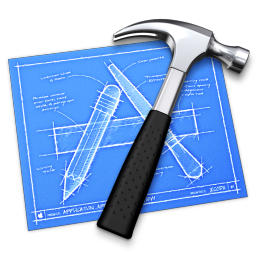
\includegraphics[keepaspectratio, height=1cm]{xcode.png}
    
\includegraphics[keepaspectratio, height=1cm]{atlassian.png}
    
\includegraphics[keepaspectratio, height=1cm]{eclipse.png}
    
\includegraphics[keepaspectratio, height=1cm]{git.png}
    
\includegraphics[keepaspectratio, height=1cm]{subversion.png}
    
\includegraphics[keepaspectratio, height=1cm]{gnu.png}
    
\includegraphics[keepaspectratio, height=1cm]{jenkins.png}
    
\includegraphics[keepaspectratio, height=1cm]{office.png}
    
\includegraphics[keepaspectratio, height=1cm]{virtualbox.png}
    
\includegraphics[keepaspectratio, height=1cm]{vmware.jpg} \\
  \end{skills}

  \resumesection{Training}
  GE Foundations of Leadership, GE Customer Technical Presentation Skills

  \resumesection{Interests}
  SW Development Process, Dev Ops, Automated Build

\end{document}
